\chapter{Executing Relay}
\label{ch:execute}

The final piece of the puzzle is taking a sufficiently
    lowered Relay program and executing it.
In theory a naive interpretation strategy could be applied
    to the entire Relay program.
In fact Relay definitional interpreter
  implements exactly this strategy,
  it just performs a straightforward recursive AST traversal.
A definitional interpreter is sufficient to
  specify the behavior of program, but not
  to efficiently execute one.
 Most compilers have a final code generation
  pipeline which transforms a generic optimized
  program to a specific backend.
Finally dynamic behaviors require
  runtime support, such as memory allocation,
  device selection, or scheduling.

The remainder of this chapter focuses on the back
  half of the Relay compiler and its runtime mechanisms.
We describe the general backend compilation strategy,
  lowering Relay to the graph runtime, the virtual machine,
  ahead of time compiler, and hardware accelerators.
In this chapter we evaluate Relay's performance specifically
  on state-of-the-art NLP applications and demonstrate
  state-of-the-art performance out performing leading industry standards
  such as TensorFlow and PyTorch.

\section{Compiler Framework}

To begin we first refresh the reader on the end-to-end
  of the Relay compiler.
First, the frontend converts input formats into the Relay IR.
Next, the Relay compiler typechecks and optimizes the program.
Processes such as automatic differentiation can be performed
  during this step.
Next we extract primitive functions
  from the Relay program, functions which may be lowering to TE or TIR,
  the process for selecting these
  is defined in Section \ref{sec:fusion}.
We then perform scheduling and lowering on these
  expressions to produce low-level target-specific versions
  of these functions.
Relay then further transforms the code which can not be lowered
  into TIR in a sequence of passes depending on which backend
  we are targeting.
Finally we execute the remaining Relay code via a TVM runtime
  either the interpreter, which directly interprets the AST,
  the virtual machine, graph runtime, or native compiler all
  of which requires separate compilation phases.
The focus of this chapter is describing this process in
  detail for each compilation and runtime target.

\subsection{Frontend}

There are several ways to write an Relay program.
A user can build an in-memory representation of
    a program in C++ or Python,
    parse one written in the Relay text format,
    load one from the on-disk serialization format,
    or import one from popular frameworks and interchange formats
    (e.g., TensorFlow, MxNet, Keras, DarkNet, and ONNX).
Many frameworks and interchange formats use static computation graph-based representations,
    which can easily be translated into Relay.
A greater challenge is translating frameworks
    with a richer computation model such as TensorFlow (TF).
TF supports control flow and includes \verb|TensorArray|, a write-once
    tensor container.
We can extract the loop structure out of a TensorFlow graph, converting
    it to an Relay loop, and transform the \verb|TensorArray| into an Relay list.
Many "importers" struggle to translate TensorFlow's full graph as their intermediate representation
  is not rich enough to capture the full IR, and often result in ad-hoc hacks to replicate
  TensorFlow's behavior.
Once new deep learning languages and IRs under development
    are stable it is likely that they can all be translated into Relay (see
    Section~\ref{sec:pl_techniques_in_dl}).
PyTorch provides an expressive programming model, and is a good fit
    for Relay, which has been previously integrated into PyTorch's
    % TODO CITE
    JIT infrastructure, enabling users to transparently use Relay for improved performance.

\subsection{Compiler}
Once an Relay abstract syntax tree (AST) is produced,
    the program is optimized by applying a series of Relay-to-Relay
    passes.
Between each pass, Relay performs type inference and checking,
    rejecting malformed programs as well as populating shape and type
    information that passes can utilize.
The Relay compiler supports traditional optimizations
    (e.g., constant folding, common subexpression elimination, and dead code elimination)
    and domain-specific optimizations, see Chapter~\ref{ch:related} for more details.

\subsection{Runtimes}

Relay produces machine-specific code
    by decomposing the problem of code generation into multiple distinct phases.
Relay translates all operators into \tvm expressions
    to produce dense linear algebra kernels~\citep{tvm_osdi18, tensor_comprehensions, halide}.
\tvm produces low-level operators that expect a fixed calling convention,
    as well as preallocated inputs and outputs.
The result is an object file containing hardware-specific implementations of all
    operations.
The remaining Relay program then is executed or compiled,
    with operator invocations replaced by calls to the optimized operators.
By representing operators as \tvm expressions, we can programmatically
    transform them and automatically generate new implementations for the transformed operators.
Optimizations like fusion and quantization
    rely on this novel behavior.
After primitive operators are lowered,
    the remaining Relay program ties
    together operator invocations, allocation, control-flow,
    recursion, and high-level data structures.
There are multiple options for executing the combined full program:
    the Relay interpreter (with JIT compilation),
    an Relay virtual machine,
    the \tvm graph runtime,
    and an experimental Relay ahead-of-time compiler
    that converts programs to C++ to produce a target-specific binary.

\section{Interpreter \& Graph Runtime}
\label{sec:interp_graph_rt}

In the tradition of definitional interpreters we introduced
  a simple interpreter for Relay which implements its formal semantics, which
  we have separately formalized.
Relay’s interpreter can execute the full language but has notable limitations
  that make it unsuited for production deployments.
It is structured as an inefficient interpreter that performs
  AST traversal to execute the program.
Each time we want to run a sub-expression we must traverse each child node
  a large cost that can be easily avoided.
Furthermore we perform JIT compilation of concrete observed shapes in the
  interpreter, a flexible, but also costly choice.
This approach is conceptually simple but inefficient, as the AST traversal heavily relies on indirection.
For example the initial Relay prototype reused the existing ``graph runtime'', to obtain
  acceptable performance for vision tasks.

The graph runtime is heavily over engineered for completely static
  models.
The graph runtime can only execute simple control-free,
    DAGs of operations.
We can optimize Relay programs and map a subset of them
    to the graph runtime, but any use of new Relay features
    are unsupported.

\section{Virtual Machine}
\label{sec:vm}

Existing approaches to dynamic model optimization apply or extend existing
  deep learning frameworks~\citep{xu2018cavs, gao2018low, yu2018dynamic, jeong2018improving, jeong2019janus, dynet, tf_fold}.
As discussed in Section~\ref{sec:dl_frameworks} frameworks are large monolithic pieces
  of software that still has serve portability and performance challenges.
Existing work which builds on frameworks extends the programming model either
`via sophisticated additions~\citep{yu2018dynamic} or significant runtime overhead~\citep{tf_fold, jeong2019janus}.
Other work~\citep{xu2018cavs, gao2018low, tf_fold} which is focused on optimizing specific types of models
  is often hard to generalize to new models, or generalize over all models.
Moreover, approaches which inherit from frameworks rely on third-party kernel libraries such as
  OpenBLAS~\citep{xianyi2014openblas}, cuDNN~\citep{cudnn}, and MKL-DNN~\citep{mkldnn} to achieve competitive performance.
These libraries expose a fixed set of operators for the corresponding hardware, compromising the portability of dynamic models
  which require a large number of operators with varying data types and shapes. Designing a new interface independent of existing frameworks
  provides a clean programming model but often at the cost of performance, due to dynamic interpretation of the model~\citep{dynet}.

However, deep learning compilers have been primarily restricted
  to static models due to lack of support for dynamism.
Specifically, in order to compile and execute the dynamic models,
  a system requires an intermediate representation (IR) which can statically represent dynamic constructs,
  a code generator which can generate kernels for dynamically varying data shapes,
  and a runtime to handle the dynamic execution and kernel dispatch accordingly.
In addition, dynamic-specific optimizations, such as dynamic memory planning, the process of statically optimizing dynamic allocations,
  are necessary to achieve desirable performance.
None of these features exist in the current deep learning compilers.

To this end, we present Relay VM, a high-performance and portable system for compiling, optimizing,
  and executing dynamic neural networks on multiple platforms.
To the best of our knowledge, this is the first attempt to systematically handle dynamic models from a compiler perspective.
First, we introduce type system extensions to handle data with unknown dimension,
  which is common in dynamic models,
  by performing type checking and inference for shapes with {\em Any}.
Second, we devise several optimizations specific to dynamic models,
  including dynamic shape-aware code generation,
  memory planning, and device placement.
Third, we propose a virtual machine (VM)-based runtime,
  which decouples the platform-independent controlling logic and platform-dependent kernel implementation,
  to be portable, light-weight, and most importantly, able to execute dynamic models.
Experimental results on LSTM~\citep{lstm}, Tree-LSTM~\citep{tree_lstm} and BERT~\citep{devlin2018bert}
  show that Relay VM~lowers the latency by 1.05$\times$ to 19.9$\times$ compared to the best solution whichever
  on mainstream hardware platforms both in the cloud (Intel CPUs and Nvidia GPUs) and at the edge (ARM CPUs).

In summary, the Relay VM is build around three core design contributions:
\begin{itemize}
  \item IR extensions for dynamical shaped tensors
  \item Optimization for internalizing Tensor memory management
  \item Designs and implements tensor based abstract machine with a platform-independent instruction set to efficiently and flexibly execute dynamic models across platforms.
\end{itemize}

\subsection{A Tensor Virtual Machine}

The first iteration of Relay defined an IR with formal semantics
  but did not provide a state-of-the-art execution mechanism (see above more discussion on this point).
For completely static models we relied on the graph runtime,
  but did not provide an efficient solution for executing
  programs beyond the reference interpreter.

Conventional deep learning runtimes, those which apply interpretation of the
  computation graph by walking each node in topological order, are non-optimal
  for dynamic neural networks.
These interpreters are reminiscent of the earliest
  languages interpreters where the input language is directly
  processed to execute the program.

By introducing models which make use of new features such
  as control flow, recursion, dynamic shapes, and dynamic allocation,
  we must change how execution works.
There are further challenges in compiling dynamic code, such as dynamic scheduling and allocation,
  fully dynamic tensor shapes, and control flow.
The interpreter offers simple solutions for these, but none is sufficiently compelling or optimized.
The simplicity of the graph runtime provides attractive
  properties such as simple serialization, straightforward
  optimal memory layout, and ease of deployment.

To address these challenges we designed a new Relay
  virtual machine.
The Relay virtual machine balances the competing approaches to execution,
  providing a dynamic execution environment which can be extended, instrumented,
  and integrated with other approaches
  like ahead-of-time compilation via flexible extension mechanisms.
The virtual machine strikes balance between performance and flexibility
  when deploying and executing Relay programs, without giving up the benefits of TVM.

Virtual machine (VM) design is a well-studied area in programming languages and systems,
  and there have been various virtual machine designs for both full-fledged and embedded programing languages.
Previous language VM designs have been heavily tailored to the execution profile of traditional programs.
Traditional programs manipulate small scalar values
  and consist of a large number of low-level instructions.
The sheer quantity of instructions requires instruction execution
  and dispatch to be extremely efficient.
In the context of machine learning we manipulate primarily tensor values,
  using a (relatively) low number of high level instructions.
ML programs’ cost centers are expensive operator invocations,
  such as GEMM or convolution, over a large input.
Due to the execution profile exhibited by ML programs,
  micro-optimizations present in scalar VMs are dramatically less important.

% The Relay virtual machine implement a simple register based VM.

% The VM consists of three pieces:
% \begin{enumerate}
%   \item A tensor instruction set for a tensor virtual machine.
%   \item A compiler from Relay to the tensor VM.
%   \item An implementation of the virtual machine.
% \end{enumerate}

In Relay, we compile a dynamic model into a {\em VM executable} which contains
  platform-independent bytecode and platform-dependent kernel code, which can be later loaded and executed.
The bytecode consists of a series of instructions that predicate the order of kernel invocation and control flow execution logic.
This design compliments conventional runtime's capability for executing highly optimized kernels but not directly handling orchestration between kernels.
Relay's instruction set is designed as an abstract machine for executing tensor valued
computations. We can realize this abstract machine by either interpreting it or generating
machine code. This is a tried and true approach utilized by existing languages and languages
runtime such as Java, or C\#.

By lowering the full language to an abstract machine we can reduce it to its core operations,
resulting in a small set of operations we can implement. Our implementation uses a virtual
machine design over an ahead of time compiler. In traditional virtual machines the key
reason to perform ahead of time compilation is to reduce dispatch time, and specialize
away dynamic features such as virtual dispatch.

Due to the design of the Relay instruction set, instruction dispatch is a very minimal
part of the total runtime, the runtime is defined by kernel execution time.
A virtual machine allows easier experimentation and modification at the cost of dynamically
dispatching instructions, though nothing in our design prevents ahead of time compilation
of the instruction set, but it provides little value for this reason.

For example if we need to produce ahead of time
compiled code, we either must generate calls into a runtime system (which is dynamic),
only removing instruction dispatch, or statically schedule limiting flexibility and
extensibility.

Furthermore our use of TVM means all kernels are ahead of time compiled meaning the
code which dominates execution time, remember most kernels are quadratic or cubic in
complexity, have efficient implementations.

Our extensions for dynamically sized kernels also utilize TVM code generation, enabling
ahead compilation of kernels which perform a form of polymorphic inline caching for shapes,
playing a similar role to what an ahead of time compiler does in traditional JITs.

Figure~\ref{fig:vm} shows the system architecture of Relay that we propose to achieve the aforementioned design goals.
It is a system consisting of two major components, namely a compiler and a runtime.
Relay takes a model in the format of mainstream deep learning frameworks, converts it into a unified intermediate representation (\textit{IR}), then optimizes and compiles the IR into an executable that contains both platform-agnostic bytecode and platform-dependent kernel code, and finally loads the executable to execute in the VM-based runtime.
%The bytecode is designed to only express the semantics of the IR, e.g. the control-flow and platform-dependent kernel invocation, through dedicated instructions, which contributes a negligible portion of the total execution time, as we will show in~\autoref{sec:eval}.
The bytecode is executed by Relay's runtime interpreter, which is shareable across various platforms.
This design effectively enables us to only maintain one version of the execution logic, but focus more on the performance critical operator kernels.
The kernels are highly-optimized for a specific hardware platform to achieve high performance.
%Kernels optimized for data with different shapes are compiled separately and dispatched accordingly.

To effectively support dynamic models without performance degradation for static models, we introduced various analysis and optimization techniques in Relay's compiler.
First, a set of IR extensions are devised to represent dynamic shapes (\textit{Any} shape) and dynamic allocations for static optimization of dynamic program behaviors (\autoref{sec:compliation:typing}).
Second, shape functions are attached to operators to compute the output shapes dynamically and perform type checking at runtime (\autoref{sec:compilation:shape-func}).
Third, a memory planning optimization is employed to reduce amount of memory consumed (\autoref{sec:compliation:memory}).
Fourth, a heterogeneous device placement mechanism is designed to place IR nodes on ``the-best'' device to reduce expensive cross-device data transferring and synchronization (\autoref{sec:compliation:hetero}).
Finally, the compiler features a code generator that is capable of specializing the code generation of certain likely shapes (\autoref{sec:compliation:codegen}). Once the executable with dynamic behavior is compiled, the VM-based runtime can load and interpret it with intelligent dynamic kernel dispatching (\autoref{sec:runtime}). We detail the design and implementation of each of these features in the followed sections.


\subsection{VM Compiler}

In order to execute on the VM we wrote a new compiler which
  can lower Relay directly on to the VM bytecode, and then
  executed.
The compiler performs a set of transformations on the high-level
  Relay program before generating code:
\begin{itemize}
  \item A-Normal Form, converts program in to a limited single-assignment form.
  \item Lambda Lift, converts inline functions into top-level definitions,
        ensuring that capture lists are now explicit.
  \item Inline Primitives, ensures that fused functions are inlined into
        the program to enables simplified code generation.
  \item Inliner, general function inlining.
  \item Constant Pool Layout, traverse program collecting all constant values
        and layout them out in memory.
  \item ADT Tag Allocation, allocate the tag assignment for compilation
        to the VM.
\end{itemize}


\subsection{VM ISA}

% \begin{itemize}
%     \item \verb|ret| Returns a value.
%     \item \verb|invoke_packed| Invoke a packed function with the specified arguments.
%     \item \verb|alloc_tensor| Allocate a tensor of the given size.
%     \item \verb|alloc_datatype| Allocate a datatype with the fields.
%     \item \verb|alloc_closure| Allocate a closure.
%     \item \verb|get_field| Project a field.
%     \item \verb|if| Conditional jump based on the condition register.
%     \item \verb|get_tagi| Get the object's tag.
%     \item \verb|fatal|
%     \item \verb|invoke| Invoke a Relay function.
%     \item \verb|invoke_closure| Invoke a Relay closure.
%     \item \verb|load_const| Load a constant from the constant pool.
%     \item \verb|int_const| Store a constant integer in destination.
% \end{itemize}

%The implementation of the VM compiler is straightforward, with the interesting design decisions found in our instruction set's design.
The design of the VM instruction set is motivated by the simple observation that kernel execution dominates neural network execution time. If we treat kernel invocation as a single instruction, the cost of surrounding instructions is negligible in the total execution.

As a result, our design is quite different from traditional language virtual machines, which contain many instructions that perform little work, leading to a profile where the cost of each instruction executed matters.
Our ISA is composed of CISC-style instructions in which each instruction corresponds to a primitive IR expression on tensors, such as allocation and kernel invocation, which in turn may correspond to executing multiple ``low-level'' operations. For example, \texttt{LoadConst idx, \$reg} is capable of multiple addressing modes as it first reads the index \texttt{idx} and then loads the data from a constant pool to the destination register \texttt{\$reg}.
A complete list of instruction set can be found in the appendices.
We naturally select a register-based virtual machine design~\citep{davis2003case} for compact a bytecode, which is easy for users to read and modify. We provide the abstraction of an infinite set of virtual registers as it significantly simplifies optimizations and allocation (similar to SSA) and minimizes conceptual barriers to rapid prototyping and modification.

Instructions are represented using a traditional tagged union containing the op-code and the data payload. This representation enables both efficient serialization and instruction decoding and dispatch. Relay uses variable-length instruction format due to the inclusion of variable sized operands such as data shapes in the instructions.

\begin{comment}
\begin{table*}[t]
\centering
\small

\begin{comment}

    \begin{tabular}{@{}ll@{}}
    \toprule
    Instruction                                                   & Description                                                                \\ \midrule
    Move                                                          & Moves data from one register to another.                                    \\
    Ret                                                           & Returns the object in register result to caller's register.                 \\
    Invoke                                                        & Invokes a function at in index.                                               \\
    InvokeClosure                                                 & Invokes a Relay closure.                                                      \\
    InvokePacked                                                  & Invokes the function containing registered operators in TOPI.                \\
    AllocStorage                                                  & Allocates a storage block.                                                  \\
    AllocTensor                                                   & Allocates a tensor value of a certain shape.                                 \\
    AllocTensorReg                                                & Allocates a tensor based on a register.                                      \\
    AllocDatatype                                                 & Allocates a data type using the entries from a register.                     \\
    AllocClosure                                                  & Allocates a closure with a lowered virtual machine function.                  \\
    GetField                                                      & Gets the value at a certain index from an VM object.                          \\
    GetTag                                                        & Gets the tag of an Algebraic Data Types (ADT) constructor.                    \\
    If                                                            & Jumps to the true or false offset depending on the condition.                 \\
    Goto                                                          & Unconditionally jumps to an offset.                                            \\
    LoadConst                                                     & Loads a constant at an index from the constant pool.                         \\
    LoadConsti                                                    & Loads a constant immediate.                                                  \\
    DeviceCopy                                                    & Copy a chunk of data from one device to another.                             \\
    ShapeOf                                                       & Compute the shape of a tensor.                                               \\
    Fatal                                                         & Raises fatal in the VM.                                                      \\
    \bottomrule
    \end{tabular}


    \end{comment}

    \begin{tabular}{@{}p{0.1\textwidth}p{0.375\textwidth}p{0.1\textwidth}p{0.375\textwidth}@{}}
    \toprule
    Instruction    & Description                                                  & Instruction   & Description.                                            \\ \midrule
    Move           & Moves data from one register to another.                     & GetField      & Gets the value at a certain index from an VM object.          \\
    Ret            & the object in register result to caller's register.          & ReshapeTensor & Changes the shape of a tensor without altering its data.      \\
    Invoke         & Invokes a function at an index.                              & If            & Jumps to the true or false offset with a condition.           \\
    InvokeClosure  & Invokes a Relay closure.                                     & Goto          & Unconditionally jumps to an offset.                           \\
    InvokePacked   & Invokes the function including operator kernel.              & LoadConst     & Loads a constant at an index from the constant pool.          \\
    AllocStorage   & Allocates a storage block.                                   & LoadConsti    & Loads a constant immediate.                                   \\
    AllocTensor    & Allocates a tensor value of a certain shape.                 & DeviceCopy    & Copies a chunk of data from one device to another.              \\
    AllocTensorReg & Allocates a tensor based on a register.                      & ShapeOf       & Retrieves the shape of a tensor.                               \\
    AllocADT.      & Allocates a data type using the entries from a register.     & Fatal         & Raises fatal in the VM.                                       \\
    AllocClosure   & Allocates a closure. & GetTag        & Gets the tag of an Algebraic Data Types (\texttt{ADT}) cstr.       \\
    \bottomrule
    \end{tabular}

\caption{The opcode and the description of the Relay instruction set \label{tab:isa}}
\end{table*}
\end{comment}

% This design has the following benefits. First, both CISC instructions and variable length encoding contribute to better code density. This is a significant advantage for edge devices that only have limited resources. Second, allowing multiple addressing modes to execute a single instruction can reduce the amount of data fetched from cache hierarchy and main memory. It may also lead to better spatial locality as the data (e.g. the tensor value) may remain in the cache. Third, a variable-length instruction encoding paves the way for extending extra information to instructions, e.g. debugging and even branch prediction. Last but not least, the instruction designed in Relay effectively separates hardware-dependent kernels from model control logic. The Relay bytecode is hardware-independent which eases bytecode serialization, and can be paired with hardware-dependent kernels being invoked by the \texttt{InvokePacked} instruction.

\subsection{Interpreter}

After we have generated a VM executable,
%\yida{we never define what is a VM executable}
we can create an interpreter by loading the executable. When execution begins, the interpreter runs a dispatch loop which checks the op-code and executes the appropriate logic, then repeats. As our instructions are coarse-grained (i.e. they can be viewed as super-instructions), the number of branches generated by the dispatch-loop is lower than traditional programming language VMs, adding negligible overhead compared to ahead of time compilation.

VM uses a tagged object representation reminiscent of those used by programming languages such as Haskell, and OCaml. The tagged object representation smoothly integrates with various data structures, including tensors, algebraic data types, and closures. Due to the specialized object representation, VM instructions only need to interact with the coarse-grained data (i.e. tensors) requiring infrequent memory allocation in chunks.

In sum, the interpreter handles instructions in the following categories.
%\yida{somewhat mention interpreter in the above two paragraphs, otherwise it feels disconnected}

\begin{itemize}[leftmargin=*]
    \item Register-to-Register Operations. Register-to-Register operations, e.g. \texttt{Move}, transfers data between different offset of the register file. Objects are reference counted, make use of copy-on-write and passed by reference ensuring register operations are cheap even if the size of underlying container is large.

    \item Memory Operations. Memory operations can allocate space for tensors, load constant tensors, and so on. Due the design of our constant pool, weights (which are constant during inference) can remain in-memory with no specialized support they can be referenced by the\texttt{LoadConst} instruction.

    \item Call Operations. Call operations are the most frequently executed instructions. The ISA
    has specialized call instructions for invoking a global function, a kernel primitive, closure, copying data across devices, reshaping runtime tensors, and calculating the shape of tensors. Kernel primitives are ahead-of-time compiled through and can leverage both compiler-generated kernels and the third-party libraries.
    %\yida{Should we briefly mention how to decide which kernels (in the context of multiple kernels) to invoke? I don't mean whether to invoke compiler-generated kernels or third-party libraries.}

    \item Control Flow Operations. Unconditional jump instructions, e.g. \texttt{ret}, are used by both static and dynamic models to jump to a specific program point. Only dynamic models need conditional control operations to determine the direction of branching. The interpreter updates the PC using the offset from either the true branch or false branch based on the conditional value.
\end{itemize}

% TODO interpreter figure

\subsection{Discussion}


The VM can be seen as the realization of a tensor abstraction machine, which corresponds to high-level tensor operations such as allocating a tensor, invoking an operation like conv2d, or performing a device copy.
An alternative solution to the VM could be ahead of time compilation from our abstract machine into machine code.
But due to the granularity of the operations, dispatch time makes up a very small portion of the execution time.
More importantly, the VM provides flexibility traditionally attributed to virtual machines and a clear compiler/runtime split.
We see the potential of VM to be integrated as a runtime module into a larger system.
For example, VM can provide resource isolation where multiple inference instances share the same hardware in the cloud.
Furthermore, a Quality of Service (QoS)-aware system, e.g., \citep{kang2018hotmobile, Yachir2009rsj}, could leverage VM to pause the
current model execution for a higher priority or time-critical model. Last, because of the simplicity of the VM design, one can verify the implementation of VM for security and privacy purposes.

Our VM is designed to execute the dynamic models by removing the limitations of the existing runtimes which only support statically shaped programs.

\section{Compiler Support for Dynamism}
\label{sec:compliation}

A key challenge preventing existing deep learning compilers from handling dynamism is the lack of a uniform and dynamic representation. For example, optimizations and runtime of existing IR, e.g., TVM \citep{tvm_osdi18}, always assume the presence of static shape information. These assumptions introduce quite a few challenges for optimization to dynamism.

In order to handle dynamism, we design a set of IR extensions which expose the essential semantics required to optimize dynamic programs. The approach is implemented in Relay VM on top of the Apache TVM (version 0.6) deep learning compiler infrastructure \citep{tvm_osdi18} to leverage its frontend converters from various DL frameworks to its IR. TVM's frontends alleviate the need to frontend specific details enabling our work to focus on contributions such as IR extensions and optimizations. To use Relay VM, one only needs to feed it with a pre-trained model, perform compilation and then inference. Furthermore, the lessons
here are applicable to other compiler efforts.
%such as TensorFlow's MLIR support or PyTorch's TorchScript and TensorExpr (a Halide and TVM inspired DSL for kernel codegen) work.

This section describes how we transform standard TVM programs into our dynamic dialect which enables us to easily apply static optimizations to dynamic programs, much as we do in traditional compiler optimization. Particularly, we detail three key components required to compile dynamic models.

\begin{itemize}
    \item An extended type system which enables static tracking of dynamic shapes.
    \item A series of optimization passes that make dynamic output shapes, allocation, and device placement explicit.
    \item A set of codegen techniques for producing code of kernels with dynamic input and output shapes.
\end{itemize}

% \vspace{-1.5em}
% \subsection{Typing}
% \label{sec:compliation:typing}
% Deep learning compilers use type systems to represent, check and infer the data types and shapes of tensors. In some frameworks and compilers this is separated into two steps, shape inference and data type inference. TVM performs both simultaneously and refers to them as type inference~\citep{roesch2019relay}, a terminology we will use throughout the section.

% A {\em Tensor Type} is designated by an $n$-dimensional shape (defined as a tuple of integers describing the tensor's dimensions) and a data type (e.g. \texttt{float32} or \texttt{int64}).
% Current deep learning IRs only support codegen when all dimensions of a tensor's shape are known at compile-time, i.e., static shapes are mandatory for type inference and checking.

% In the context of dynamic models, many data shapes can only be determined at runtime. Therefore, the previous assumption of static data shapes does not hold.
% In order to support dynamic data shapes, Relay VM introduces a special dimension called \any~to represent statically unknown dimensions.
% For example, we can represent a tensor type as \texttt{Tensor[(1, 10, Any), float32]},
% where the size of the third dimension in this tensor is unknown while the other
% two dimensions have concrete values.
% This concept has been introduced in other frameworks.
% Janus \citep{jeong2019janus} uses similar denotation to represent a dynamic dimension but only for type unification, while Relay VM extends type inference to handle \any~as described next. %We do not support tensor types with dynamic ranks given the relatively limited use cases and optimization opportunities.
% %\yida{Do we need the following sentence?}The challenge of introducing a dynamic shape extension is adapting each layer of the system to handle it in a way that does not greatly degrade performance.

% \noindent
% {\bf Operator Type Relation} A type relation describes the relationship between types of operator inputs and outputs. The type system of TVM relies on these type relations to infer and bidirectionally propagate type and shape relationships between inputs and outputs of operators across the whole network.
% %For example, the type relation for broadcasting operators (e.g. \texttt{broadcast\_add}) performs the shape calculation following the NumPy broadcasting rules.

% The type relation must be generalized to properly handle dynamic shapes. For example, a program which grows a tensor on each loop iteration (a case existing in the decoder of many NLP models) is both impossible to type and compile without proper type system support. With the introduction of \any, we are able to improve the existing type relations to support dynamic models.

% There are two dynamic type relation cases in particular.
% First, operators with dynamic output shapes depending on the input data, such as {\tt arange}\footnote{{\tt arange} generates a range of values in a (start, stop, step) interval the arrays output size is a function of input arguments.} and {\tt unique}\footnote{{\tt unique} selects the unique elements of a tensor.}, will use \any~to describe those shapes.
% % We can now describe the type relation using the enhanced type relation functions with \any but not before.
% % For example, type relation of {\tt arange} can be expressed as follows
% % \[
% % arange: fn(start: fp32, stop: fp32, step: fp32) \rightarrow \langle [\any], fp32 \rangle
% % \]
% Second, when input shapes contain \any~dimension, the type relation needs to propagate \any~correctly to the output types and relax typing constraints that hold in the static cases when necessary.
% %For example, type relation for {\tt broadcasting} operators determines the compatibility between corresponding dimensions from both inputs if they are equal or one of them is 1 according to the Numpy broadcasting rule.
% For example, the rules
% for broadcast\footnote{\url{https://docs.scipy.org/doc/numpy/user/basics.broadcasting.html}} type relation with \any~are defined as follows:
% %\vspace{-1em}
% \begin{align*}
%   \textrm{broadcast\_rel}(\any, 1) &\rightarrow \any \\
%   \textrm{broadcast\_rel}(\any, d) &\rightarrow d ~~~~~~(d > 1) \\
%   \textrm{broadcast\_rel}(\any, \any) &\rightarrow \any
%   \vspace{-1em}
% \end{align*}
% %\vspace{-1em}
% Note that due to the presence of dynamic shapes, these type relation rules can no longer rule out all type errors at compile-time.
% For example, for the second rule shown above, when \any~is neither 1 nor $d$ at runtime, it then violates the broadcast type constraints.
% To address this, we take the gradual typing~\citep{gradualtyping} approach and leave certain type checking at runtime after \any~is instantiated by a
% concrete value (see \autoref{sec:compilation:shape-func} for more details).
% One could eliminate these errors using a more advanced type system, but at increased complexity.

% \noindent
% {\bf Type Inference} One caveat of the \any~dimension is that unknown dimensions will propagate during type inference, reducing chances for shape specialization.
% For example, if we use an operator such as {\tt arange} to produce a tensor with dynamic shape (i.e., \texttt{Tensor[(\any,), float32]}) and later {\tt broadcast\_add} to a tensor with static shape (i.e., \texttt{Tensor[(5, 1), float32]}), the output shape will also contain an \any~dimension (i.e., \texttt{Tensor[(5, \any), float32])}.

% To limit the contamination of \any, we further introduce {\em sub-shaping} to improve the precision of types computed by type-inference.
% Much like sub-typing used in popular programming languages \citep{LiskovTPLS1994,AmadioAmadioTPLS1993}, our extension enables values with more specific shape information to be passed in contexts which require less specific shapes.
% Further, we perform extra analysis that repeatedly replace one \any~dimension by a symbolic variable followed by a type inference pass to identify if other \any~dimensions share the same symbolic expression.
% %on each \any~dimension to detect if two \any~dimensions point to an identically sized dimension.
% This information is passed to downstream compilation and can reduce the search space during the symbolic codegen.
% %We can use this analysis in the downstream compilation to generate shape-specialized code during codegen.

% % We treat concrete dimension and symbolic dimension as a sub-shape of \any.
% % \yida{The following sentence is problematic with grammatical error. We need to explicitly define what is an argument.}Rules for invoking a function, suppose fn type is $fn\langle T_1, \dots, T_n\rangle$,
% % and arguments are $T'_1, \dots, T'_n$, the rules are defined as follows
% % \begin{align*}
% %   \textrm{union}(T_i, T'_i) &\rightarrow T_i \\
% %   \textrm{join}(T_i, T'_i) &\rightarrow T'_i
% % \end{align*}
% %\vspace{-1em}

% %\vspace{-1em}
% \subsection{Shape Function}
% \label{sec:compilation:shape-func}
% %Existing deep learning compilers only deal with static shapes, enabling all shape computation to occur at compile-time.
% %Therefore, it is easy to allocate memory for the tensors using static shape information to compute the precise amount of storage needed for each tensor.
% %However, introducing \any~invalidates this pre-allocation mechanism as the tensors may now contain dynamic dimensions.
% The introduction of \any~dimension invalidates the pre-allocation mechanism adopted in the existing deep learning compiler.
% Instead, we now have to track the amount of memory required to be allocated in parallel to computing.
% Furthermore, static type checking cannot eliminate all type errors at compile-time due to dynamic tensor shapes.
% Consequently, we define a {\em shape function} to compute the output shape for storage allocation and verify the type relation in accord with the semantics of every operator.
% The shape function is similar in structure to the type relations described in \autoref{sec:compliation:typing} but are present at runtime instead of compile-time.
% It enables compiling and embedding the computation of output shapes into the program.

% According to the characteristics of the operator, we divide the shape functions in three different modes: data independent, data dependent, and upper bound.
% {\em Data independent} shape functions are used for operators in which the output shape only depends on the shapes of inputs such as normal 2-D convolution.
% {\em Data dependent} shape functions require the concrete input values to compute the output shapes. For example, the output shape of \texttt{arange} depends on the value of start, stop, and step.
% In addition, there are certain operators such as Non Maximum Suppression (\texttt{nms}) where the complexity of computing the output shapes is on par with the complexity of executing the operator itself.
% In order to avoid the redundant computation, we use an {\em upper bound} shape function to quickly estimate an upper bound shape for the output.
% We also require such operators to return the output shape along with output value, so as to use the real shape to slice the output tensors into precise output shape and layout.
% %\yida{use a diagram to summarize three modes and remove the text}

% It is worth noting that in the presence of dynamic shape functions, operator fusion needs to be specially taken care of.
% Operator fusion, which combines {\em basic operators} into a {\em composite operator}, is a critical technique for performance optimization as it reduces unnecessary memory copies and improves the cache locality.
% %However, we only define the shape function at elementary operator level. As a result, we also must fuse shape functions in parallel with the operator fusion.
% The compiler can easily connect the shape functions of basic operators to form the shape function for a composite operator when all shape functions are data independent.
% However, a basic operator with a data dependent or upper bound shape function cannot be fused to other operators, i.e., taking the outputs of other operators as its inputs to fuse together, as the shape function requires to access to the intermediate result within a composite operator.
% As a result, we explicitly define the fusion policy to prevent this from happening.
% %If all basic ops in a composite op have data independent shape functions, it is straightforward to generate shape function for this composite op as we can just connect the shape functions of basic ops together. However, a composite op is invalid if a basic op that has a data dependent or upper bound shape function takes the intermediate output of another basic op as input.
% %Because the intermediate result in a composite op is inaccessible from outside, the data dependent shape function cannot collect all arguments it required. Thus, we revise the operator fusion policy correspondingly to make sure composite ops generated by the operator fusion pass will be valid.

% %Due to our definition of shape functions we are able to perform fusion using a generalized version of the algorithm used for standard operator fusion which handles passing the appropriate input shape or input depending on the shape function. For example imagine that the fuse operator has a single input that was originally used an operator that requires the input, and the second fused operator requires the input shape. Depending on the type of the shape function defined above, we handle operator fusion in the following manner. Any data independent shape functions could be fused with other operators. Any fused group can only have at most one shape function and it should be fused together with the operator that needs shape function.

% \input{mlsys/memory}

% \vspace{-1em}
% \subsection{Heterogeneous Device Placement}
% \label{sec:compliation:hetero}
% As discussed in \autoref{sec:compilation:shape-func}, shape functions are executed at runtime to calculate the output shape of an operator. These functions should execute on the CPU as their outputs are used to compute the size of allocated memory. In the case of heterogeneous execution (i.e., CPU and GPU), it is essential to carefully place the execution of IR nodes to proper devices. Otherwise, considerable overhead from data transfers and device synchronization will occur if the inputs to shape functions and kernels need to be copied from or to GPU. To minimize the performance penalty, we analyze the program to place sub-expressions on the most suitable devices.

% We introduce a unification based analysis for computing the correct device placement and allocation based on the previous scheduling of the compute kernels. The goal of our device analysis is to assign each IR node properly to minimize the number of cross-device copies. We introduce a concept of \texttt{DeviceDomain} to represent the domain of a device, including source and destination. Each expression in the IR defaults to the empty domain, meaning no constraint on its device placement. In addition, a new IR construct, \verb|device_copy|, is introduced to facilitate the heterogeneous execution of the Relay VM runtime. It represents a data transfer between different devices and is inserted when a cross-device data copy is mandatory.
% %The latter\yida{what does this refer to?} is used to retrieve the shape of a tensor at runtime and is used to efficiently compute the input shapes for shape functions.
% Our analysis is formulated as a set of device placement rules which describes how device constraints flow, and then we use unification, a technique common in type inference and compilers, to compute the precise device placement.
% \autoref{fig:hetero} depicts some highlights of the rules to assign and propagate the device types: (a) both inputs and outputs of shape function are assigned to CPU, (b) the output of \verb|device_copy| is assigned to the device that is copied to, (c) all arguments to \verb|invoke_mut| should have the same device domain. The full set of rules can be found in the \autoref{appx:hetero-rules}.

% \begin{figure}
%     \centering
%     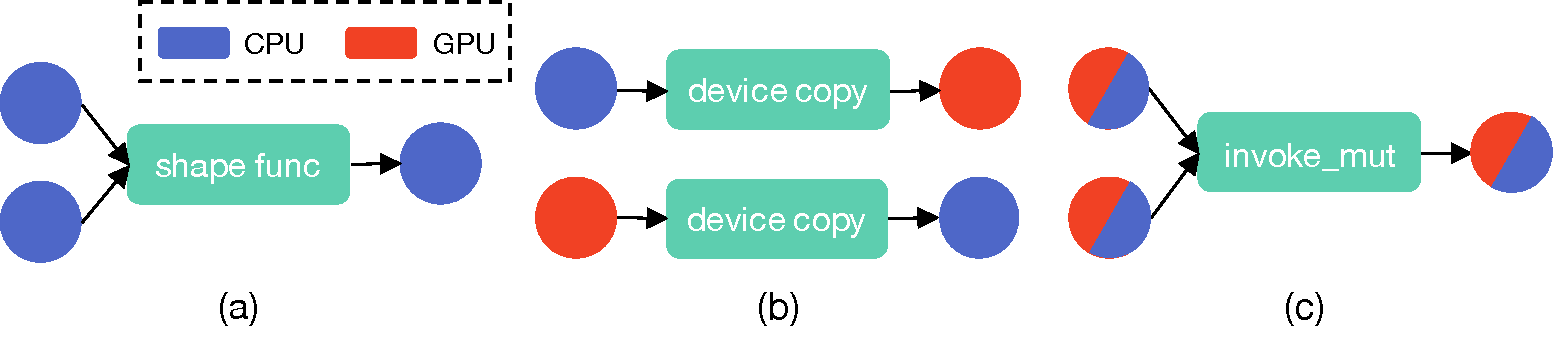
\includegraphics[width=\linewidth]{figs/hetero.pdf}
%     \caption{Some heterogeneous device placement rules. (a) The inputs and outputs of shape functions are placed on CPU.
%     (b) \texttt{device\_copy} changes the device of output accordingly.
%     (c) The device of all arguments to \texttt{invoke\_mut} must be the same.
%     }
%     \label{fig:hetero}
%     \vspace{-2em}
% \end{figure}

% Based on these rules, we use a union-find data structure to bidirectionally propagate and unify the device placement of each IR node. We introduce two operations, \texttt{union(s, t)} and \texttt{find(s)}, to achieve \texttt{DeviceDomain} unification throughout the entire program. \texttt{union(s,t)} unions the equivalence device domains of \texttt{s} and \texttt{t} into one equivalence domain when the device types match. \texttt{find(s)} returns the representative of the device domain that \texttt{s} belongs to. These two operations are applied until all IR nodes are annotated. The result of the heterogeneous device placement composes with memory planning and shape function insertion resulting in correctly placed allocations.

% \vspace{-1em}
% \subsection{Symbolic Codegen}
% \label{sec:compliation:codegen}
% %\yida{Should we mention the mechanism of invoking third-party libraries in this subsection?}
% Deep learning compilers~\citep{tvm_osdi18, halide} have demonstrated competitive performance compared to manually tuned kernels on multiple platforms. Recent trends apply machine learning based search to further reduce or eliminate complex manual performance tuning using either template based~\citep{chen2018learning, zheng2020flextensor} or search based~\citep{adams2019learning, zheng2020ansor} approaches.
% However, existing work which focuses on tuning in the presence of static shapes falls short with symbolic or dynamic shapes. There are two inherent challenges with regard to codegen of symbolic shapes.
% %\begin{itemize}
% %    \itemsep 0em
% \squishlist
%     \item How to achieve the same performance of kernels generated with symbolic shapes as that with static shapes when applying the same schedule?
%     \item How to extend the machine learning based approach to tune kernels with symbolic shapes?
% \squishend
% \vspace{-1em}
% %\end{itemize}

% Loop parallelism and loop tiling are common optimization techniques that exploit multi-core capabilities by achieving data access patterns which are memory hierarchy aware for both CPUs and GPUs. However, the combination of these techniques lead to complex loop boundary conditions. In many static cases, it is possible to prove these conditions always hold, and thus eliminate checks which hamper further optimizations such as unrolling.
% While straightforward to handle with static shapes, it becomes a non-trivial challenge when performing symbolic codegen. If not carefully handled, the boundary condition checks will stay, leading to poor performance.

% To address this issue, we generate multiple kernels according to the residues modulo of the tiling factor and then dispatch based on the actual shape at runtime.
% For example, suppose a symbolic dimension $x$ is tiled by a factor of 8, we then duplicate the generated kernel for 8 times, and replace the symbolic var $x$ by $8k+r$ in each copy, where $k = \lfloor x / 8 \rfloor$ and $r \in [0..7]$. By applying this technique in conjunction with an enhanced symbolic expression simplification pass, we can eliminate most boundary checks to achieve performance that is nearly identical to kernels compiled with a single static shape. Lastly, we automatically generate a dispatch function that invokes the corresponding kernel based on the residue.
% %because this function is also generated in the IR we can compile and optimize it like other code ahead of time.
% In addition, the dispatch function can be extended to invoke either compiler generated kernels or {\em third party library} whichever is faster from the profiling results.
% The increased kernel size is relatively small compared to the overall deep learning models.
% In case where resources are extremely limited, we can either generate fewer number of kernels than the tiling factor or reduce the tiling factor to find an acceptable trade-off between code size and performance.

% A known issue to machine learning based tuning is that it may take a long time (usually hours) to find the best schedule for a single kernel. When it comes to symbolic shapes, the tuning time may be exponentially longer if we naively tune for every possible shape. In this paper, we extend the template based tuning approach for symbolic shapes to make tuning time tractable. The template based tuning approach takes a human-defined code template and a search space, and searches the best configuration within the search space by using machine learning algorithms.
% %by building on the techniques explored in based~\citep{chen2018learning}.
% We observe that a good configuration for one shape usually performs well on other shapes. Based on this observation, we devise the following mechanism to tune the kernel for symbolic shapes.

% \vspace{-12pt}
% \begin{enumerate}[leftmargin=*]
%     \itemsep 0em
%     \item First replace the symbolic dimensions by a large enough value (e.g., 64) so that the search space can cover most possibilities, and run the tuning algorithm on the static shape for a sufficient number of iterations.
%     %\vspace{-8pt}
%     \item Pick top $k$ configurations, apply them to a selection of other shapes, and evaluate their performance.
%     %\vspace{-8pt}
%     \item Pick the configuration that performs best on average among shapes previously evaluated.
% \end{enumerate}
% \vspace{-12pt}

% Empirically, we found that $k=100$ covers most of the best configurations for other shapes. Current popular dynamic models usually only require kernels with one symbolic variable. As a result, we choose the values of power of two up to 256 in the cross evaluation of other shapes. If there is more than one symbolic variable, a more sophisticated selection approach might be required to limit the evaluation time of step 2. We leave this to the future work. Further, if the workload distribution is known, we can adjust the weighting of known shapes in step 3.

% %Though we address both challenges, we admit that our approach has limitations when all dimensions are unknown. In these cases symbolic codegen cannot completely replace manually tuned 3rd party libraries yet, but is complimentary when partial shapes are known.\yida{Can we remove this paragraph?}

% % Our codegen approach for dynamic shapes is designed to integrate well with TVM's codegen. We implement a bucketing
% % based codegen strategy, which generates a set of shape-specialized variants and code which selects between them. One
% % attractive consequence of this design is that it allows us to integrates with the current version of AutoTVM~\citep{chen2018learning}, TVM's auto-tuning framework
% % to further optimize kernels.

% % When an operator appears with dynamic shape it often will only vary along a single dimension. We are able to handle cases that
% % deal with imperfect tiling strategies but the critical performance piece is choosing a tuned operator with the appropriate tile size.
% % We reuse the machinery of the VM to support invoking a bucketed operator. For each operator with a dynamic shape we will
% % generate tile sizes for powers of two, and then for a given input size round to the nearest power of two tile size and select that operation.
% % The code for selecting between buckets is also realized as TVM expression allowing further optimization of the combined kernel.
% % This strategy can be viewed as a form of polymorphic inline caching~\citep{inline_caches}, where the cache is not keyed by type, but shape.

% % The bucketing strategy we employ obtains
% % For this paper we explored one possible strategy for generating code but using the infrastructure of this paper
% % it is relatively low cost to explore new strategies by reusing the machinery.


\subsection{Ahead-of-time}


\section{Supporting Hardware Accelerators}
\label{sec:accel}

\subsection{Bring Your Own Code Generation}

In conjunction with my collaborators at AWS we implemented an
  extensible framework for hooking hardware accelerators into
  TVM.
Bring Your Own Code Generation (BYOC) is a mechanism introduced
  into Relay for offloading specific sub-programs to hardware
  accelerators which operate outside of the traditional TVM
  programming model.


\subsection{VTA}

Hardware specialization is a powerful way to accelerate
  a known set of applications and workloads.
A component of Relay is lowering high-level programs down
  to the bespoke semantics of emerging hardware accelerators.
Unfortunately, deep learning (DL) is anything but a static field, and the machine learning (ML) community
  rapidly changes how they use to write models, the architecture of models themselves, the operators
  used by said models, and the data types they operate over.
Initial programmable accelerators~\citep{tpuv1} offer potentially huge performance
  improvements at the cost of complex specialized compilation.
Furthermore the churn of machine learning has lead to an interest
  in customizable designs, with features such as new numeric representations,
  new hardware engines, and more.
In order to customize the behavior of accelerators designs, even when open-sourced,
  there is a need for the availability of a transparent and modular software stack.
An end-to-end approach requires integration of frameworks, systems, compilers,
  and architecture in order to execute state-of-the-art ML using hardware acceleration.
Peak FLOPs provide value only if a programmer can access them.
In order to tackle this problem I have collaborated on the design for \vta (Versatile Tensor Accelerator),
  an explicitly programmed accelerator paired with a compiler and runtime that can evolve
  in tandem with deep learning models without sacrificing the advantages of specialization.

\vta makes following contributions:

\begin{itemize}
    \item \emph{A programmable accelerator design} that exposes a two-level programming interface: a high-level task ISA to allow explicit task scheduling by the compiler stack, and a low-level microcode ISA to provide software-defined operational flexibility.
    In addition, the \vta architecture is fully parameterizable: the hardware intrinsics, memories, and data types can be customized to adapt the hardware backend requirements.
    \item \emph{An extensible runtime system} for heterogeneous execution that performs JIT compilation of microcoded kernels to provide operational flexibility. For example, the \vta runtime lets us extend the functionality of \vta's original computer-vision-centric design to support operators found in style transfer applications without requiring any hardware modifications.
    \item \emph{A schedule auto-tuning platform} that optimizes data access and reuse in order to rapidly adapt to changes to the underlying hardware and to workload diversity.
\end{itemize}

My collaborators and I published a paper on VTA in
  the IEEE Micro Journal Special Issue on Deep Learning Acceleration.
\vta and its children projects are a critical part of the research
  agenda at UW SAMPL lab, and we won a multi-million dollar grant to
  pursue automatically mapping Relay programs to hardware designs.
This work is being continued at UW and its one exciting future
  direction we discuss in Chapter~\ref{ch:future}.
